\chapter{Method}
\section{Choice of Method}
\label{sec:choiceOfMethod}
The main research question of this study was used to determine which research method would be the most fitting. The following is the question we arrived at:

\begin{itemize}
\item How do organizations perform information security incident management in practice?
\end{itemize}

Figure \ref{fig:methods} shows an overview of various research methods and three criteria that can be used to determine the appropriate research method for a study. The criteria are: form of research question, whether the study requires control of behavioural events and if the study focuses on contemporary events. The defined research question for this study is a so-called "how" question. The goal was to reveal current practices in organizations and the study did therefore not require control of any behavioural events. The study focuses mainly on contemporary events. Some past events such as incidents that have occurred are relevant, but the main focus is on current practices. Based on this, case study emerged as the most suitable method for this study, as shown in the figure.

There are other advantages to choosing case study as the research method for this study. Case studies can provide information that can help judge if specific technologies will benefit an organization or project \cite{kitchenham1995case}. This is applicable to our study and especially to the sub-question:

\begin{itemize}
\item To what extent are existing standards/guidelines adopted in plans for information security incident management?
\end{itemize}

This question seeks to identify if standards/guidelines are used and if they benefit an organization.

\begin{figure}[H]
\begin{center}
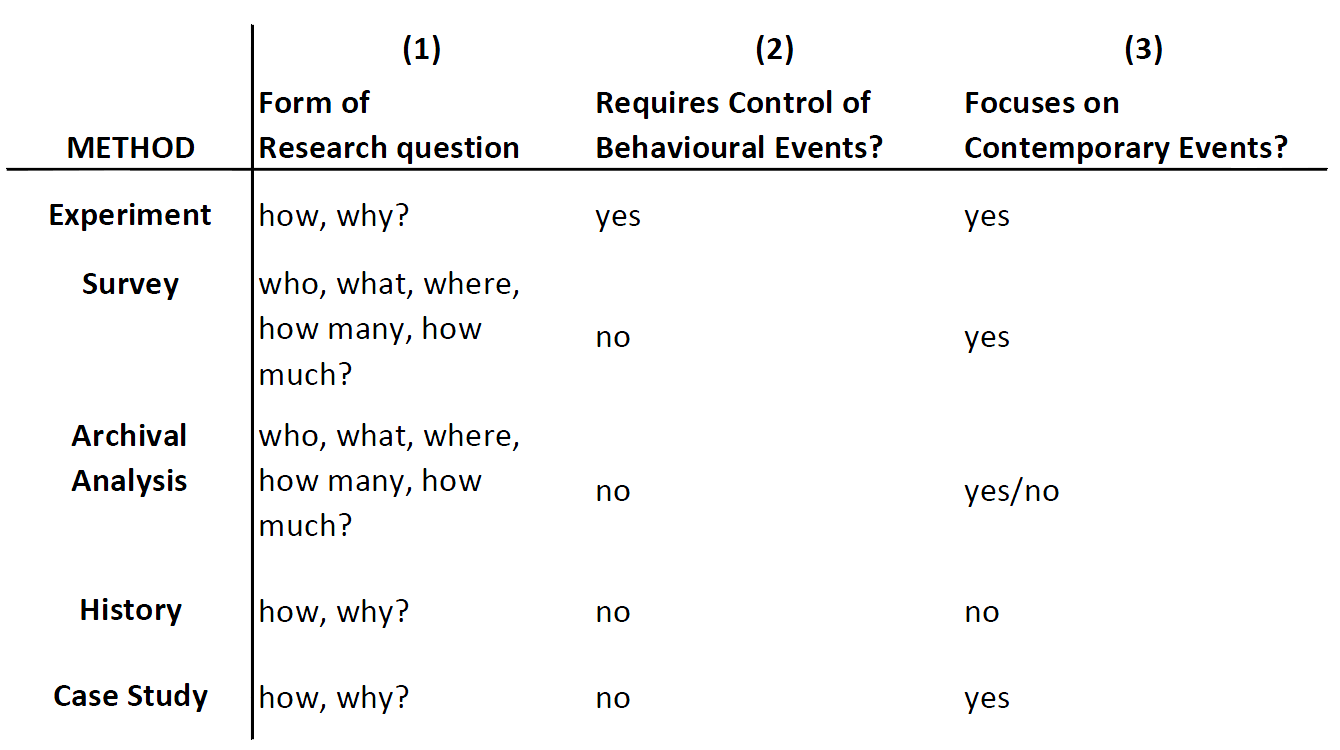
\includegraphics[scale=0.35]{methods.png}
\caption[Situations for different research methods]{Situations for different research methods, modified from \cite{CaseStudyResearch}}
\label{fig:methods}
\end{center}
\end{figure}

A case study is applicable to real-world projects, which is what we wanted to study. Another important advantage is that it can deal with various kinds of evidence, such as documents, archival records, interviews and artefacts.

\section{Qualitative research}
We used a qualitative research method where we focused on relatively few informants. Unlike a quantitative approach where using questionnaires to gather information from a large number of participants is common, we wanted in-depth information from selected organizations. Using a qualitative research method enabled us to do rich and detailed analysis. 

Further, we followed an inductive research approach. In inductive research, researchers perform field studies followed by deriving theories from observations. This method is a contrast to deductive research where a theory is developed initially, followed by observations to evaluate it\cite{oates2005researching}. 

\textbf{Deductive research:} The researcher's objective is to test a theory or hypothesis using new empirical data. This approach is known as \emph{theory-testing} research\cite{bhattacherjee2012social}.

\textbf{Inductive research:} The researcher's objective is to infer theories and patterns from observed data. Also called \emph{theory-building} research\cite{bhattacherjee2012social}.

As inexperienced researches we chose an inductive research approach as we felt it gave less bias in our research. Hence, we aimed at starting our observations with an open mind instead of working towards proving a specific theory. Three main objectives for inductive research are; to compress the extensive amount of data gathered through a qualitative study into a summary, to establish links between research objectives and elements from the findings and finally to develop theories or models about the underlying structure of experience which are found in the data\cite{thomas2006general}.

\section{Case Study}
\label{sec:caseStudy}
This section describes case study as the chosen research method for this thesis. The content is derived from \cite{CaseStudyResearch} where Yin defines a case study in the following way:

\paragraph{Case Study:} An empirical inquiry that investigates a contemporary phenomenon in depth and within its real-life context.

%\begin{itemize}
%\item A case study is an empirical inquiry that investigates a contemporary phenomenon in depth and within its real-life context, especially when
%\item the boundaries between a phenomenon and context are not clearly evident.
%\end{itemize}
%\item The case study inquiry
%\begin{itemize}
%\item copes with the technically distinctive situation in which there will be many more variables of interest than data points, and as one result
%Hva er variables og hva er data points?
%\item relies on multiple sources of evidence, with data needing to converge in a triangulating fashion, and as another result
%\item benefits from the prior development of theoretical propositions to guide data collection and analysis.
%\end{itemize}
%\end{enumerate}

The case study inquiry relies on multiple sources of evidence and benefits from the prior development of theoretical propositions to guide data collection and analysis.

The research process is illustrated in figure \ref{fig:caseProcess}. As the figure shows, the process in linear, but iterative. This means that one can go back to previous phases if needed. The Plan phase consisted of identifying research questions and deciding to use case study as the research method for this study. The Design phase is about getting from initial questions to conclusions or answers. It is the logic that links the data to be collected to the initial questions of the study. 

\begin{figure}[h]
\begin{center}
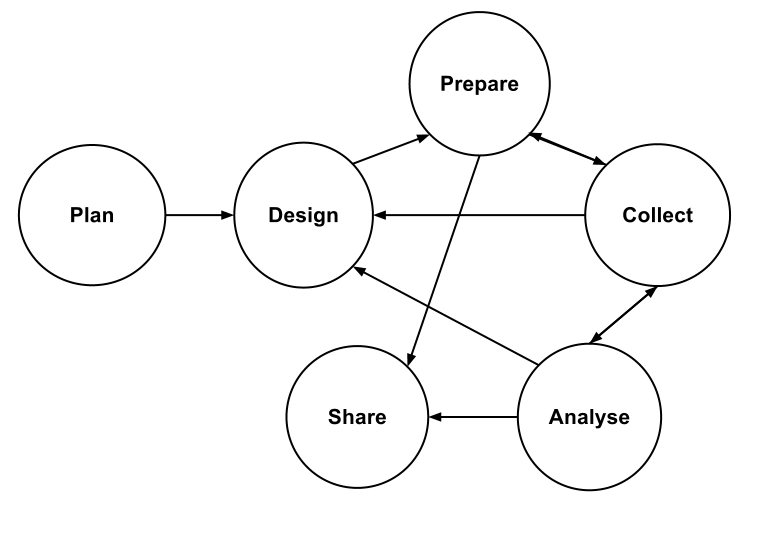
\includegraphics[scale=0.38]{caseProcess.png}
\caption[Case Study Research Process]{Case Study Research Process \cite{CaseStudyResearch}}
\label{fig:caseProcess}
\end{center}
\end{figure}

Yin presents tactics to maximize the quality of empirical research. He recommends to use multiple sources of evidence and to have key informants review a draft of the report. Both of these tactics were used in this study. 

The choice between a single- and multiple-case belongs to the Design phase. Multiple-case is usually preferred and was chosen as the method for this study. Additionally each case may be embedded or holistic. An embedded case has more than one unit of analysis. The design for this study is a mix. It is a multiple-case study where one case has three embedded units of analysis and two cases are holistic. The design of our study is illustrated in figure \ref{fig:caseDesign}.

\begin{figure}[ht]
\hspace{-0.28cm}\includegraphics[scale=0.375]{caseStructure.png}
\caption[Case Design for This Study]{Case Study Design, modified from \cite{CaseStudyResearch}}
\label{fig:caseDesign}
\end{figure}

The Preparation phase was very important as we did not have experience with the case study research method. The main activities performed in this phase were acquiring desired skills to become case study investigators and preparing for the specific case studies. It is considered difficult to obtain these skills as procedures are not routinised. It is advised to prepare to ask good questions, be a good ``listener", be adaptive and flexible, have a firm grasp of the issues being studied and be unbiased by preconceived notions. We have performed a background study in order to get a thorough understanding of the issues in the study. Relevant background information is discussed in chapter \ref{chp:background} and the background study itself is briefly discussed in section \ref{sec:background}. %Develop a protocol for the investigation? screen candidate cases? Pilot case? No..

Interviews, documents and surveys were chosen as the sources of information in the Collection phase. The use of multiple sources of evidence is consistent with the definition of a case study, which is presented in the beginning of this section. The interview is seen as being one of the most important sources of information in a case study. Documentary information is likely to be relevant in any case study. These data collection methods are described and discussed in sections \ref{sec:interviews}, \ref{sec:documentStudy} and \ref{sec:employeeSurveys}.

The Analyse phase is described in section \ref{sec:qualitativeAnalysis}.

The Share phase consisted of preparing, writing and editing this report. Choices such as to anonymize identities of individuals and individual organizations were part of this phase. This choice is further discussed in section \ref{sec:ethical}. It was a choice that was made as part of the preparation of the study and this illustrates the arrow from Prepare directly to Share, and shows that the case study process is not purely linear. 

\subsection{Background Study}
\label{sec:background}
The first step in our research were a background study of security incident management. In order to find appropriate questions for the interviews we found it necessary to study relevant literature such as standards and best practice guidelines. We focused on the well-established and internationally accepted ISO/IEC standards in addition to documentation from the \ac{NIST}.

We also looked at related work and what have been studied earlier in the field of incident management. In this way the background study was used to guide the data collection. It was also used in the data analysis, by comparing standards and prior developed theory tot he findings of this study. This is consistent with the definition of a case study, as presented at the beginning of section \ref{sec:caseStudy}.

\subsection{Qualitative Interviews}
\label{sec:interviews}
We chose to perform qualitative interviews in our research as they are common and powerful tools to gather information in qualitative research\cite{myers2007qualitative}. The goal of qualitative interviews is to see the research topic from the interviewee's perspective and understand why and how they got that particular perspective\cite{cassell2004essential}. To meet this goal, qualitative interviews are driven by open questions and a low degree of structure and often focus on specific situations and experiences made by the interviewee. 

We used what is referred to in literature as semi-structured interviews\cite{cassell2004essential}. We wanted interviewees to talk freely about their experiences, and thus we did not follow a strict order of predefined questions. However, to ensure we got all information required to answer our research questions we used an interview guide. The interview guide works as an incomplete script and states the main goals for our research as well as the main research questions and topics for the interview.

The interview questions were not asked in any particular order, but rather when found appropriate to ensure a smooth dialogue. This gave opportunities to ask follow-up questions. When using semi-structured interviews, interviewees can be seen as being ``participants" in the research, rather than someone who only answers pre-defined questions.

We performed the interviews face-to-face voice recorded the dialogue. By conducting interviews face-to-face we hoped to build trust with the interviewee and thus get better and more elaborative answers. It also gave us opportunity to explain and elaborate questions that were unclear. Since we recorded all of the interviews we could focus on listening and thus ask the best follow-up questions instead of being extracted by writing answers. Also, we could listen to the recordings several times as needed and clarify things that were unclear later.

Developing an interview guide, carrying out interviews and analysing them can be highly time-consuming activities. Participating in interviews is also time-consuming for interviewees, which could have made it challenging to recruit interviewees for our study. One mitigation to the risk of not recruiting interviewees was sending out letters explaining the main purpose of our research, what was expected by the interviewee, and how the interviews would play out. We also notified organizations at an early stage and set dates for the interviews to ensure their commitment.

Qualitative interviews are very flexible as they can be used to tackle various forms of research questions related to organizations. Despite the time effort spent on developing an interview guide, questions and conducting the interviews, we found qualitative interviews to add great value and thus the most suited for our research.

\subsection{Document Study}
\label{sec:documentStudy}
There are both advantages and disadvantages to document-based evidence. Documentation is stable, it can be reviewed repeatedly, it is not created as a result of the case study and may have broad coverage. However it can be difficult to find, biased selectivity may occur, there may exist some unknown bias of the author and some documents may be deliberately withheld. In this study, some of these disadvantages are attempted mitigated by trying to find all relevant documentation and by informing the participants of the data handling process and that sensitive information would not be revealed to any other party than the students and their supervisors. The latter was to try to avoid documentation being withheld.  

%\section{Action Research}

\subsection{Qualitative Data Analysis}
\label{sec:qualitativeAnalysis}
%Hvordan gikk vi fra raadata til konklusjon?\\
%grupperte ut fra forskningssporsmaal? faser i standarder? caser?\\
%saa etter patterns? connections between segments?\\
%explain patterns, kan noe relateres til tidligere teorier? Se paa flere ulike men mulige forklaringer paa funene.

Advantages:
Gives a rich and detailed analysis
Could be more than one "correct" solution or theory based on various objects of analysis.
Important to evaluate ones sources.

Disadvantages:
The interpretation of data is based on researchers background.
The amount of data can be challenging.

\textbf{Generalisation:}

%Se google docfil

\begin{figure}[H]
\begin{center}
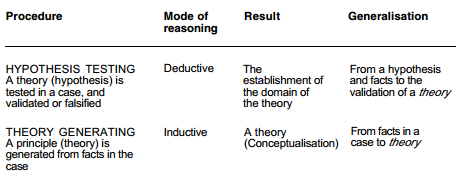
\includegraphics[scale=0.9]{ModesOfGeneralisation.png}
\caption[The modes of generalisation]{The modes of generalisation, modified from \cite{johansson2003case}}
\label{fig:modesofgeneralisation}
\end{center}
\end{figure}

\section{Participants}
%In the nature of qualitative research participants were chosen to be diverse such that different perspectives on incident management (in the same context) could be studied.large organizations that are likely to have experiences severe security incidents. + de i Gjovik gjorde paa small/medium.. her gjor vi en dybdestudie av noe annet!Hvorfor de vi valgte? Hvorfor er de interessante?

\section{Ethical Considerations}
\label{sec:ethical}
%Litt i forhold til at man behandler sensitiv information og saann
The main ethical concern related to our research is the potentially confidential information revealed during interviews. Organizations unlikely want details about their information security practice to become public. Hence, no names are mentioned in this report that could identify participating organizations or individuals.

Since a voice recorder was used during interviews, participants could potentially be identified later by voice recognition. Participants were given information about how collected data was handled through a statement of consent and were also given the right to withdraw from the study at any given time. This project was reported to the Norwegian Social Science Data services. The information sheet, including the statement of consent can be found in Appendix A (in Norwegian).  

signere konfidensialitetserklaering?


\subsection{Anonymization}
\section{Challenges}
This case study relies on qualitative information and a challenge related to that is to work hard to report all evidence fairly. Additionally this type of research provides little basis for scientific generalization. \cite{CaseStudyResearch}.

For quantitative data there exist clear convention for analysis, but there are fewer guidelines for the analysis of quantitative data. In relation to this Allen S. Lee states in \cite{lee1989scientific}, ``but the analyst faced with a bank of qualitative data has very few guidelines for protection against self delusion".

Basing most of our information gathering on interviews, the challenges with this approach had to carefully considered. The authors had little or no experience in preparing and conducting qualitative interviews. Michael D. Myers and Michael Newman discusses potential challenges with using qualitative interviews in\cite{myers2007qualitative}. 

They mention the artificiality of qualitative interviews where one interrogates a stranger that does not know or trust you. The lack of trust may cause the interviewee to withhold information that could be of value to the study. As an attempt to mitigate trust issues the procedure of handling data (anonymization) was presented as well as highlighting that the project had been reported to the Norwegian Social Science Data Services.   

Problems could also arise if too little time is assigned for the interviews. Questions could be rushed causing inaccurate information or that important information are left out. To avoid time limitations being a concern, we assigned more time than estimated for each interview. We also used the interview guide with predefined questions and topics as well as correcting any misunderstandings during the interview to avoid ambiguous questions.

When relying on qualitative interviews for information, one have to consider potential interviewee bias as for instance security incident management knowledge vary greatly among employees in an organization. In addition, Myers and Newman mentions the possibility for interviewees to construct knowledge to appear knowledgeable and rational. By giving interviewees enough time to answer questions and carry out interviews as a dialogue, we hope to have avoided these problem.



